\documentclass{beamer}
\usepackage{inconsolata}
\usepackage{caption}
\usepackage{color}
\usepackage{listings}
\usepackage{subfig}
\usepackage{cooltooltips}
\usepackage{hyperref}
\usepackage{perpage}
\usepackage[normalem]{ulem}
\setbeamertemplate{navigation symbols}{}%remove navigation symbols
\usepackage{listings}
\usepackage{color}
\usepackage{framed}

\definecolor{background}{RGB}{39, 40, 34}
\definecolor{string}{RGB}{230, 219, 116}
\definecolor{comment}{RGB}{117, 113, 94}
\definecolor{normal}{RGB}{248, 248, 242}
\definecolor{identifier}{RGB}{166, 226, 46}



\lstset{
  language=C,               			% choose the language of the code
  alsolanguage=Python,            			% choose the language of the code
  alsolanguage=Java,            			% choose the language of the code
  numbers=none,                   		% where to put the line-numbers
  stepnumber=1,                   		% the step between two line-numbers.        
  numbersep=5pt,                  		% how far the line-numbers are from the code
  extendedchars=true,
  numberstyle=\tiny\color{black}\ttfamily,
  backgroundcolor=\color{background},  		% choose the background color. You must add \usepackage{color}
  showspaces=false,               		% show spaces adding particular underscores
  showstringspaces=false,         		% underline spaces within strings
  showtabs=false,                 		% show tabs within strings adding particular underscores
  frame=single,
  framerule=0pt,
  tabsize=4,                      		% sets default tabsize to 2 spaces
  captionpos=n,                   		% sets the caption-position to bottom
  breaklines=true,                		% sets automatic line breaking
  breakatwhitespace=true,         		% sets if automatic breaks should only happen at whitespace
  title=\lstname,                 		% show the filename of files included with \lstinputlisting;
  basicstyle=\color{normal}\tiny\ttfamily,					% sets font style for the code
  keywordstyle=\color{magenta}\tiny\ttfamily,	% sets color for keywords
  stringstyle=\color{string}\tiny\ttfamily,		% sets color for strings
  commentstyle=\color{comment}\tiny\ttfamily,	% sets color for comments
  emph={True, False, format_string, eff_ana_bf, permute, eff_ana_btr, KeyError,
  ValueError, ZeroDivisionError},
  emphstyle=\color{identifier}\tiny\ttfamily,
  morekeywords={with, as}
}

\lstset{literate=%
   *{0}{{{\color{cyan}0}}}1
    {1}{{{\color{cyan}1}}}1
    {2}{{{\color{cyan}2}}}1
    {3}{{{\color{cyan}3}}}1
    {4}{{{\color{cyan}4}}}1
    {5}{{{\color{cyan}5}}}1
    {6}{{{\color{cyan}6}}}1
    {7}{{{\color{cyan}7}}}1
    {8}{{{\color{cyan}8}}}1
    {9}{{{\color{cyan}9}}}1
}



\newenvironment{enum}{
\begin{enumerate}
  \setlength{\itemsep}{1pt}
  \setlength{\parskip}{0pt}
  \setlength{\parsep}{0pt}
}{\end{enumerate}}

\hypersetup{
  colorlinks=true,
  urlcolor=pink,
}

\MakePerPage{footnote}

\title{Python 101}
\subtitle{Lec -1 \\ Real Life Applications}
\author{thoum}

\begin{document}
\frame{\titlepage}

\begin{frame}
\frametitle{Why Python}
One of the reasons we learn Python is the various libraries others have written
  for Python.\\ We don't have to start from scratch.
\end{frame}

\begin{frame}
\frametitle{Why Python}
Numpy: Calculation\\
OpenCV: Image Processing\\
Request: Web crawling\\
Keras: Machine Learning\\
KoNLPY: Korean Natural Language Processing\\
Ren'Py: Visual Novel Engine\\
\ldots you name it.
\end{frame}

\begin{frame}
\frametitle{Today's topic}
Parse tweets on twitter, use bag of words model, so that it can be the
  basis for many possible applications.
\end{frame}

\begin{frame}{Tweepy}
  Learning how to use external libraries by reading their documents is
  important.\\
  \href{https://tweepy.readthedocs.io/en/latest/streaming\_how\_to.html}{How to
  get twitter live stream}
\end{frame}

\begin{frame}{TL;DR?}
  I provided a skeleton code with explanations.\\
  \href{https://github.com/indiofish/python\_tutor/blob/master/lec08/tweet.py}{Download}
\end{frame}

\begin{frame}{I want more than names and texts}
  \href{https://developer.twitter.com/en/docs/tweets/sample-realtime/api-reference/get-statuses-sample}{Other
  fields}
\end{frame}

\begin{frame}{Run It!}
\end{frame}

\begin{frame}{Saving?}
  Look up:
  \href{https://www.google.com/search?q=python+save+list+as+file}{saving
  files}
\end{frame}

\begin{frame}{Bag of Words}
  \begin{center}
  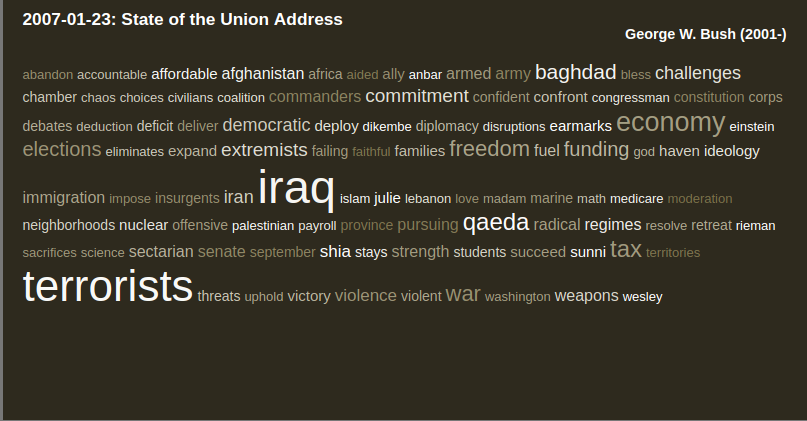
\includegraphics[width=80mm]{./bow.png}
  \end{center}
\end{frame}

\begin{frame}{Bag of Words Model}
  Ignore order of the text. Focus on word count.\\
  Simple yet strong; good for document classification.($e.g.$ spam filtering)\\
  What class can we use?
\end{frame}

\begin{frame}{The Crude Version}
  We can split our text by spaces, get word count.\\
  We can look at most common words, number of positive words, number of
  negative words... yada yada to analyze sentiment on that topic.($e.g.$ Todays
  weather? Stock? Politicians?)
\end{frame}

\begin{frame}{Try It!}
  Get the top 5 most common words related your query.(Don't forget to exclude
  the query itself; it will \textit{always} be included.)
\end{frame}

\begin{frame}{For the Future: The Improved Version}
  Unlike English, Korean vocabs are not simply split by spaces.\\
  Try this: \href{https://konlpy-ko.readthedocs.io/ko/v0.4.3/}{KoNLPy}
\end{frame}

\begin{frame}{Useful References for the Future}
  Multiprocessing in Python : Useful if you need speed.\\
  Request Module : Useful when interacting with websites.\\
  Time Complexity : Useful if you want to analyze your code.\\
  \href{https://acmicpc.net}{Baekjoon} : Useful if you want to practice some
  language or algorithms.\\
  \href{https://www.google.com}{Google} : Can't stress enough.\\
  \href{https://www.stackoverflow.com}{StackOverFlow} : Can't stress enough.\\
\end{frame}

\end{document}
